%iffalse
\let\negmedspace\undefined
\let\negthickspace\undefined
\documentclass[journal,12pt,onecolumn]{IEEEtran}
\usepackage{cite}
\usepackage{amsmath,amssymb,amsfonts,amsthm}
\usepackage{algorithmic}
\usepackage{graphicx}
\usepackage{textcomp}
\usepackage{xcolor}
\usepackage{txfonts}
\usepackage{listings}
\usepackage{enumitem}
\usepackage{mathtools}
\usepackage{gensymb}
\usepackage{comment}
\usepackage[breaklinks=true]{hyperref}
\usepackage{tkz-euclide} 
\usepackage{listings}
\usepackage{gvv}       
\usepackage{circuitikz}
%\def\inputGnumericTable{}                                 
\usepackage[latin1]{inputenc}                                
\usepackage{color}                                            
\usepackage{array}                                            
\usepackage{longtable}                                       
\usepackage{calc}                                             
\usepackage{multirow}                                         
\usepackage{hhline}                                           
\usepackage{ifthen}                                           
\usepackage{lscape}
\usepackage{tabularx}
\usepackage{array}
\usepackage{float}


\newtheorem{theorem}{Theorem}[section]
\newtheorem{problem}{Problem}
\newtheorem{proposition}{Proposition}[section]
\newtheorem{lemma}{Lemma}[section]
\newtheorem{corollary}[theorem]{Corollary}
\newtheorem{example}{Example}[section]
\newtheorem{definition}[problem]{Definition}
\newcommand{\BEQA}{\begin{eqnarray}}
\newcommand{\EEQA}{\end{eqnarray}}
\newcommand{\define}{\stackrel{\triangle}{=}}
\theoremstyle{remark}
\newtheorem{rem}{Remark}

% Marks the beginning of the document
\begin{document}
\bibliographystyle{IEEEtran}
\vspace{3cm}

\title{2018-AE-14-26}
\author{AI24BTECH11011 - Himani Gourishetty}
\maketitle
\bigskip

\renewcommand{\thefigure}{\theenumi}
\renewcommand{\thetable}{\theenumi}
\begin{enumerate}
\item A jet aircraft is initially flying steady and level at its maximum endurance condition. For the aircraft to fly steady and level, but faster at the same altitude, the pilot should
\begin{enumerate}
    \item increase thrust alone
    \item increase thrust and increase angle to attack
    \item increase thrust and reduce angle to attack
    \item reduce angle of attack alone
\end{enumerate}
\item The pilot of a conventional airplane that is flying steady and level at some altitude, deflects the port side aileron up and starboard aileron down. The aircraft will then
\begin{enumerate}
    \item pitch, nose up.
    \item roll with the starboard wing up.
    \item pitch, nose down.
    \item roll with the port wing up.
\end{enumerate}
\item A NACA 0012 airfoil has a training edge flap. The airfoil is operating at an angle of attack of 5 degree with un-deflected flap. If the flap is now deflected by 5 degrees downwards, the $c_L$ versus $\alpha$ curve
\begin{enumerate}
    \item shifts right and slope increases.
    \item shifts left and slope increases.
    \item shifts left and slope stays the same
    \item shifts right and slope stays the same.
\end{enumerate}
\item An airplane requires a longer ground roll to lift-off on hot summer days because
\begin{enumerate}
    \item the thrust is directly proportional to free-stream density
    \item the thrust is directly proportional to weight of the aircraft
    \item the lift-off distance is directly proportional to free-stream density
    \item the runaway friction is high on hot summer days
\end{enumerate}
\item The velocity profile is an incompressible, laminar boundary layer is shown in the figure below. U is the free-stream velocity, $u\brak{y}$ is the stream-wise velocity component. The area of the black shaded region in the figure below represents the 
\begin{figure}[!ht]
\centering
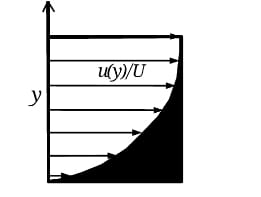
\includegraphics[width=0.3\linewidth]{figs/fig1.png}
}%
\end{figure}
\begin{enumerate}
    \item boundary layer thickness
    \item momentum thickness
    \item displacement thickness
    \item shape factor
\end{enumerate}
\item The tangential velocity component $'V'$ of a spacecraft, which is in a circular orbit of radius $'R'$ around a spherical Earth$\brak{\mu = GM\rightarrow\text{gravitational parameter of Erth}}$ is given by the following expression
\begin{enumerate}
    \item $V=\sqrt{\frac{\mu}{2R}}$
   \item $V=\sqrt{\frac{\mu}{R}}$
   \item $V=\frac{2\pi}{\sqrt{\mu}}R^{\frac{3}{2}}$
   \item $V=\frac{2\pi}{\sqrt{\mu}}R^{\frac{2}{3}}$
\end{enumerate}
\item Equation of the trajectory of  a typical space object around any planet, in polar coordinates $\brak{r,\theta}\brak{\text{i.e. a general conic section geometry}}$, is given as follows. h is angular momentum, $\mu$ is gravitational parameter , $e$ is the eccentricity, $r$ is radial distance from the planet center, $\theta$. is the angle between vector $\vec{e}$ and $\vec{r}$.
\begin{enumerate}
    \item $r=\frac{\frac{h^2}{\mu}}{1-e\cos\theta}$
     \item $r=\frac{\frac{h^2}{\mu}}{e-\cos\theta}$
    \item $r=\frac{\frac{h^2}{\mu}}{1+e\cos\theta}$
     \item $r=\frac{\frac{h^2}{\mu}}{e+\cos\theta}$
\end{enumerate}
\item In an elliptic orbit around any planet, the location at which a spacecraft has the maximum angular velocity is
\begin{enumerate}
    \item apoapsis
    \item periapsis
    \item a point at $+45^\degree$ from periapsis
    \item a point at $-90\degree$ from apoapsis.
\end{enumerate}
\item The pitching moment of a positively cambered NACA airfoil about its leading edge at zero-lift  angle of attack is
\begin{enumerate}
    \item negative
    \item positive
    \item indeterminate
    \item zero
\end{enumerate}
\item In a low-speed wind tunnel, the angular location(s) from the front stagnation point on a circular cylinder where the static pressure equals the free-stream static pressure, is
\begin{enumerate}
    \item $\pm38^\degree$
    \item $\pm30^\degree$
    \item $\pm60^\degree$
    \item $\pm0^\degree$
\end{enumerate}
\item A thermocouple, mounted flush in an insulated flat surface in a supersonic laminar flow of air measures the 
\begin{enumerate}
    \item static temperature
    \item temperature greater than static but less than total temparature
    \item total temparature
    \item temparature greater than total temparature
\end{enumerate}
\item A shock wave is moving into still air in a shock tube. Which one of the following happens to the air ?
\begin{enumerate}
    \item static temperature increases, total temperature remains constant
    \item static temperature increases, total temperature increases.
    \item static temperature increases, total temperature decreases
    \item static pressure increases, total temperature remains constant
\end{enumerate}
\item The highest limit load factor experienced by a civil transport aircraft is in the range
\begin{enumerate}
    \item 0.0-2.0
    \item 2.0-5.0
    \item 5.0-8.0
    \item 8.0-10.0
\end{enumerate}
\end{enumerate}
\end{document}a
